\documentclass{article}
\usepackage[utf8]{inputenc}
\usepackage[margin=0.675in]{geometry}
\usepackage{amsmath}
\usepackage{graphicx}
\usepackage{float}
\usepackage{hyperref}
\usepackage{listings}

\graphicspath{{images/}}
\title{Report for Assignment - Link Layer\\
CS3543 - Computer Networks - 2}
\author{Vishwak Srinivasan\\
\texttt{CS15BTECH11043}}
\date{}

\begin{document}
\maketitle 

\begin{flushleft}
Below is the protocol hierarchy using which some of the information for the next few questions were obtained:
\begin{figure}[H]
\centering
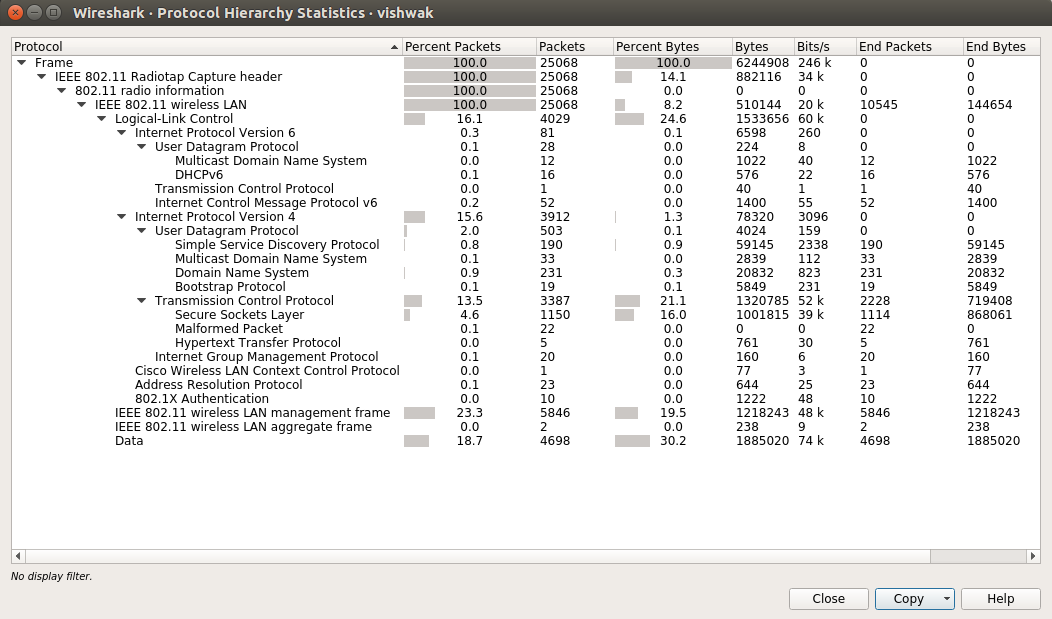
\includegraphics[width=0.7\linewidth]{protocol-hierarchy.png}
\end{figure}
\end{flushleft}

\section{Packet classification: Control, Data and Management}
\begin{flushleft}
Approximately 25000 packets were captured over Wi-Fi with multiple hosts in the network. Below are the counts and fractions:
\begin{center}
\begin{tabular}{|c|c|c|}
\hline
Class & Number of Packets & Fraction of Packets \\
\hline
\hline
Control & 4029 & 0.161 \\
\hline
Data & 4698 & 0.187 \\
\hline
Management & 5846 & 0.233 \\
\hline
\end{tabular}
\end{center}
\end{flushleft}

\section{Packet types: \texttt{ARP}, Broadcast, \texttt{TCP}, \texttt{UDP}, \texttt{ICMP(v6)} and \texttt{IGMP}}
\begin{flushleft}
Below are the counts and fractions for the different types:
\begin{center}
\begin{tabular}{|c|c|c|}
\hline
Type & Number of Packets & Fraction of Packets \\
\hline
\hline
\texttt{ARP} & 23 & 0.0009 \\
\hline
Broadcast & 5187 & 0.207 \\
\hline
\texttt{TCP} & 3390 & 0.135 \\
\hline
\texttt{UDP} & 531 & 0.0212 \\
\hline
\texttt{ICMP(v6)} & 52 & 0.0021 \\
\hline
\texttt{IGMP} & 20 & 0.0008 \\
\hline
\end{tabular}
\end{center}
Broadcast message were filtered using the filter \texttt{wlan.da == ff:ff:ff:ff:ff:ff}.
\end{flushleft}

\section{Unique users using MAC addresses}
\begin{flushleft}
For this, I had to add two new fields \texttt{Dest-MAC} and \texttt{Src-MAC}, and had to export it to a CSV. From there, I used Pandas, a Python library to extract the distinct MAC addresses which were both destination and source. There were 19 of them, which is displayed below:
\begin{figure}[H]
\centering
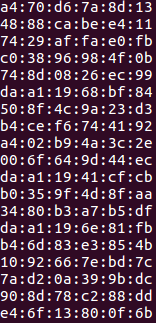
\includegraphics[width=0.25\linewidth]{users-mac.png}
\end{figure}
The source code is:
\begin{lstlisting}[basicstyle=\footnotesize\ttfamily, showstringspaces=false, language=Python]
import pandas as pd
data = pd.read_csv(`MAC-dest-src.csv', sep=`,', usecols=[`Dest-MAC', `Src-MAC'])
u_set = set(data[`Dest-MAC'].tolist()) & set(data[`Src-MAC'].tolist())
print("\n".join(list(u_set)[1:]))
\end{lstlisting}
\end{flushleft}

\section{Traffic Pattern}
\begin{flushleft}
This was done using IO graph, which revealed the packet variation with wall-clock time:
\begin{figure}[H]
\centering
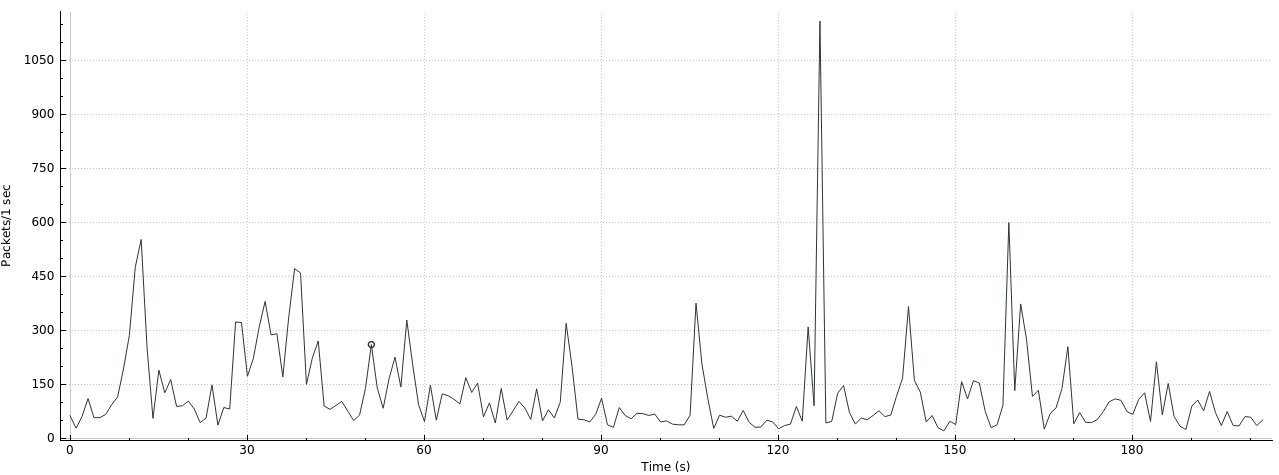
\includegraphics[width=0.75\linewidth]{traffic-pattern-l2.png}
\end{figure}
\end{flushleft}

\section{Number of ``special" retransmission}
\begin{flushleft}
The number of these retransmissions not accompanied by a link-layer ACK can be found using the filter \texttt{wlan.lc.retry eq 1}. Out of around 25000 frames, 1329 frames where ``specially" retransmitted. Below is the snapshot:
\begin{figure}[H]
\centering
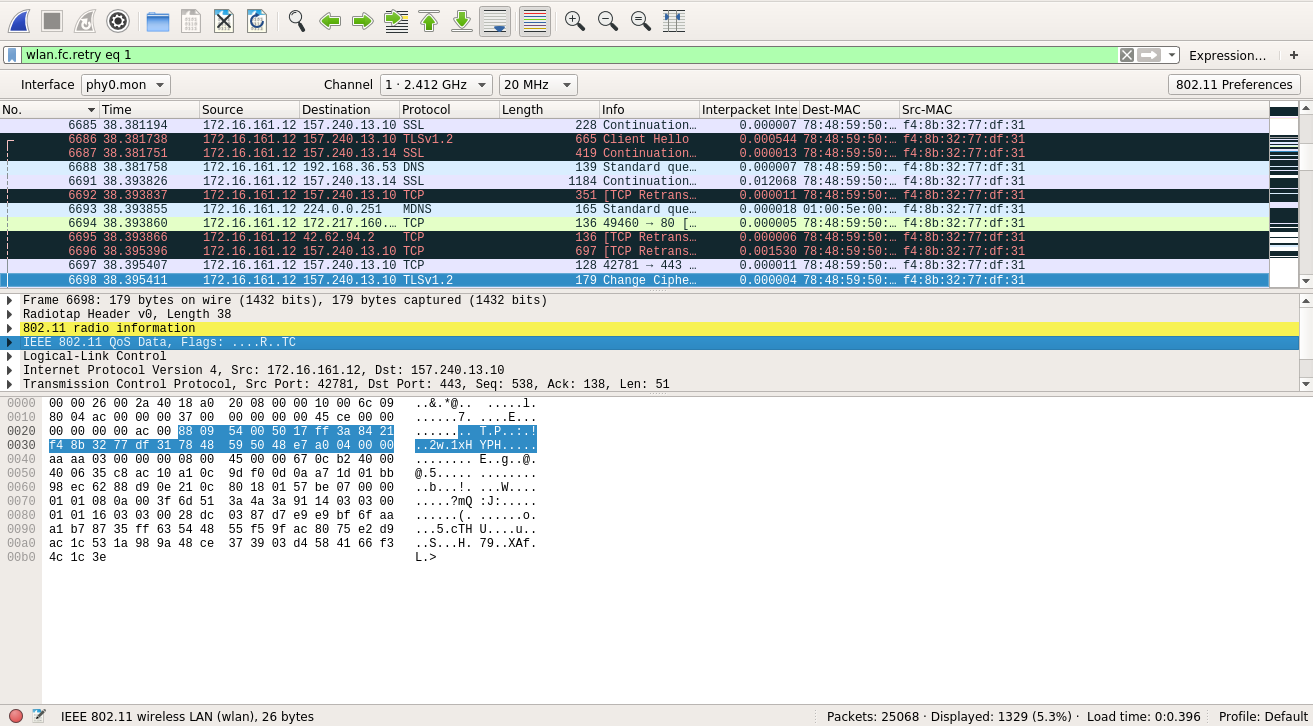
\includegraphics[width=0.85\linewidth]{snapshot-retrans.png}
\end{figure}
\end{flushleft}
\end{document}
